\chapter{Discussion}

Dans le chapitre précédent, une réflexion a été menée sur les freins à la réinsertion professionnelle des personnes en situation de handicap. Cette partie a pour but de répondre à la problématique de ce projet à travers deux questions principales :
\begin{enumerate}
\item Pourquoi encourager l'emploi des personnes handicapées en pleine conjoncture défavorable ?
\item Comment lutter contre les facteurs de résistance à la reprise de l'emploi ?
\end{enumerate}



\section{Pourquoi encourager l'emploi des personnes handicapées en pleine conjoncture défavorable ?}

Actuellement, l'emploi n'est pas à son point fort. Quand le taux de chômage pour les personnes non handicapées se positionne à hauteur de 9 \%, le taux de chômage des personnes handicapées est doublé\footnote{19 \% selon l'Agefiph : \url{http://www.agefiph.fr/L-Agefiph/Qui-sommes-nous} - Nos Chiffres clés}.\\

Bien que la crise économique ne favorise pas l'embauche de personnes (handicapées ou non), de nombreux arguments existent pour démontrer que l'employabilité d'une personne handicapée est bénéfique autant pour cette personne que pour l'entreprise. Dans cette partie, nous allons définir des arguments (sociaux, économiques et psychologiques) pour appuyer cette vérité.

\subsection{Arguments sociaux}

\subsubsection{Retrouver une vie sociale}
Pour contrer la monotonie d'une chambre d'hôpital ou la solitude d'un appartement vide, il a été démontré que retrouver une vie professionnelle pour une personne handicapée, conduit à une vie sociale plus riche.
Un sentiment de frustration peut également être présent lorsqu'une personne handicapée travaillait avant son accident.\\

Les nombreuses rencontres eues avec des personnes handicapées, lors des acculturations de l'association HandiManagement, montrent que l'ambiance de travail est également plus conviviale au sein du bureau. En effet, de manière générale, une personne handicapée qui recouvre son travail est beaucoup plus motivée qu'une autre personne.

\subsubsection{S'adapter à son handicap}
Selon une enquête portée par l'association Comète France, près de 84 \% des personnes handicapées, après leur accident, se disent limités dans la nature du travail qu'ils peuvent réaliser. Ce sentiment de limitation dans la vie professionnelle traduit la manière dont la personne envisage son devenir et se projette dans l'emploi.\\

L'intervention de structures d'aides comme Comète, leur permet d'une part de rechercher des emplois et de se rendre compte qu'ils peuvent être réinsérés professionnellement. D'autre part, cette intervention permet une restitution de la confiance. 
La reprise du travail sera accompagnée pour que la personne ne développe pas un sentiment d'inaptitude au travail, qui l'amènerait à ne plus rechercher d'emploi ou à perdre son emploi actuel.


\subsection{Arguments économiques}

Outre les aspects sociaux qui conduisent une personne handicapée à retrouver une vie sociale et à tendre vers une meilleure autonomie, des aspects économiques entrent également en jeu pour encourager l'emploi des personnes handicapées.

\subsubsection{Pour le patient}
L'accès à un salaire convenable est un facteur important à la reprise d'un travail.\\

On pourrait se demander si le facteur économique est vraiment pertinent pour une personne handicapée, compte tenu du fait qu'elle reçoit des allocations d'aide (cf Partie \ref{allocationsAide}). En effet, la reprise d'emploi entrainera, soit la suppression, soit une forte diminution du montant de ces aides, ce qui peut représenter un frein pour la personne handicapée à être employée.\\
Cependant, selon une étude de Comète France, les deux-tiers des personnes handicapées concernées par la réception d'une aide financière, ont déclaré que les aides les ont effectivement aidés à retravailler.\\

Outre le salaire qui augmentera, le travailleur handicapé pourra recommencer à économiser pour sa retraite.


\subsubsection{Pour l'employeur}
En employant des personnes en situation de handicap, l'employeur voit son nombre de personnes handicapées augmenter dans son entreprise et ainsi, la taxe versée à l'Agefiph diminuer.\\

C'est aussi un ressort très appréciable pour renvoyer au salarié valide l'image d'une productivité et d'une efficience importante fournies par les personnes en situation d'handicap.

\subsection{Arguments psychologiques}
Un sentiment d'auto-satisfaction va se développer lors de la reprise du travail, du fait que la personne retrouve une vie professionnelle, comme avant l'accident.\\

L'impact familial est également très important sur la motivation d'une personne handicapée. La personne sera alors confrontée à un sentiment d'auto-valorisation au niveau de son statut dans la famille lorsqu'elle retrouvera un travail.





\section{Comment lutter contre les facteurs de résistance à la reprise de l'emploi ?}

Encourager l'emploi des personnes handicapées s'avère crucial pour que ces dernières retrouvent une vie épanouie et une qualité de vie appréciable. Cependant, il est nécessaire de lutter contre les freins à la reprise de l'emploi détaillés en partie \ref{resultats}.\\
Les actions menant à cette insertion professionnelle doivent \^etre menées des deux c\^otés : à l'attention de l'employeur dont c'est le r\^ole d'embaucher des personnes en situation d'handicap ; et à l'attention de la personne handicapée qui souhaite retrouver un emploi.

\subsection{Du c\^oté de l'employeur}

\subsubsection{Rappeler le dispositif de législation}
Chaque entreprise est au courant du dispositif de législation qui s'applique en vigueur en France. Les entreprises qui atteignent un quota de moins de 6 \% de personnes handicapées doivent payer une contribution à l'Agefiph. Les autres entreprises ne payent pas de contribution et sont, au contraire, aidés par l'Agefiph qui leur fournit des prestations et des services.\footnote{\url{http://www.agefiph.fr/L-Agefiph/Que-faisons-nous/Nos-aides-financieres-et-services}}

\subsubsection{Sensibiliser à l'existence des dispositifs facilitant l'intégration}
Pour sensibiliser les entreprises au dispositif de législation, aux mesures facilitant l'intégration et pour effacer les préjugés, des campagnes de sensibilisation sont proposées aux entreprises, afin de les encourager à embaucher des personnes en situation d'handicap.\\

Par exemple, CapEmploi propose dans ses services des sessions de sensibilisation pour l'employeur et pour les équipes de travail qui proposent de réfléchir sur \footnote{La liste complète est disponible à l'adresse \url{http://www.capemploi.net/nous-connaitre/nos-services/}} :
\begin{itemize}
\item Le cadre juridique dans lequel s'inscrit l'employabilité des travailleurs handicapées
\item La dédramatisation du handicap (à travers des actions de sensibilisation aux différents handicaps existants)
\item La relation entre le Handicap et le poste de travail
\item Les mesures facilitant l'intégration des personnes handicapées
\item Les aménagements de poste\\
\end{itemize}

Ces actions vont dans le sens d'une meilleure compréhension du Handicap qui est un processus dynamique (comme vu dans la partie \ref{handicap_emploi}). Si une personne handicapée se sent mieux dans son environnement, son intégration sera plus aisée. Cette meilleure compréhension des facteurs variables au sein de l'entreprise conduira à une diminution du handicap lors de la réalisation de ses t\^aches au travail.

\subsubsection{Lutter contre les stéréotypes et les préjugés}

Un stéréotype est une idée, une opinion, acceptée sans réflexion et répétée, sans avoir été soumise à un examen critique, par un personne ou par un groupe, et qui détermine, à un degré plus ou moins élevé, ses manières de penser, de sentir et d'agir~\cite{handicapEntrepriseContraintes}.
La conséquence des stéréotypes est une généralisation abusive d'une idée. 
Dans ce témoignage, un chef d'une entreprise industrielle du secteur de l'énergie pensait que le recrutement de personnes handicapées n'était pas envisageable parce que son bâtiment ne possédait pas d'escaliers. Il partait de l'idée qu'une personne handicapée est forcément en fauteuil roulant. Or parmi l'ensemble des personnes handicapées, près de 3 \% sont effectivement en fauteuil roulant. Ce responsable avait donc développé un stéréotype basé sur le fait qu'il ne pourrait jamais embaucher de personnes handicapées. Alors qu'il pouvait embaucher près de 97 \% de personnes handicapées pour lesquelles prendre les escaliers n'était pas un problème.\\

Plus généralement, on remarque que le stéréotype le plus commun pour le milieu du handicap est de croire que le handicap est toujours visible. Or, près de 80 \% des personnes handicapées ont un handicap invisible. Les handicaps psychiques (dépression, schizophrénie, etc.), cognitifs (dyslexie...), mentaux ou sensoriels sont souvent des handicaps invisibles.


\subsubsection{Sensibiliser les employeurs sur la force productive des personnes handicapées}

De nombreux préjugés sévissent encore autour de la force productive et de l'efficience professionnelle des personnes handicapées. Par exemple, l'emploi de personnes handicapées peut \^etre considéré comme trop contraignant. Un autre exemple consistera à penser qu'une personne handicapée est moins productive qu'un individu valide. Si on peut dire que certains handicaps créent un écart de productivité, on ne peut pas généraliser ce propos à l'ensemble des handicaps. \\

Différentes mesures ont été mises en place (expliquées en partie \ref{mesuresIncitatives}) pour inciter les entreprises à employer des salariés handicapés.\\

Outre ces mesures, il ressort souvent des entretiens réalisés avec des personnes handicapées qu'elles travaillent d'abord pour obtenir une reconnaissance sociale, ensuite pour gagner en autonomie. Ainsi, montrer qu'elles sont aussi \textit{capables} qu'une personne valide sont un élément qui les motivent à exercer une activité professionnelle et à augmenter leur niveau de productivité.\\

Enfin, les campagnes de sensibilisation portées par l'Agefiph, le réseau Comète ou CapEmploi par exemple, aident à effacer les préjugés sur les personnes handicapées et à définir l'insertion professionnelle des personnes handicapées comme une force pour l'entreprise, et non une faiblesse.



\subsubsection{Vers une discrimination positive ?}
L'existence des préjugés et stéréotypes à l'égard des personnes handicapées conduit vers une discrimination négative : le refus d'insérer des personnes handicapées en entreprise. Cependant, il existe également l'effet inverse qui va consister à vouloir embaucher des personnes handicapées, quelque soit leurs compétences.\\

Comme les entreprises sont contraintes à un taux d'emploi de 6 \% de personnes handicapées, on pourrait croire qu'une discrimination positive a lieu (bien qu'interdite par la loi) pour atteindre le quota.\\

Pourtant la discrimination positive est à éviter car elle regroupe plusieurs problèmes.
D'une part, elle fait passer au deuxième plan les compétences de la personne. En effet, la personne a été choisie par l'entreprise parce qu'elle était handicapée. 
D'autre part, elle conduit à des échecs de l'équipe de travail et notamment de la personne handicapée qui ne trouve pas de véritable place dans l'entreprise.\\
Certaines personnes handicapées se voient donc favorisées par la direction de l'entreprise car elles sont handicapées, ce qui réduit l'équité existant entre les employés. En effet, l'entreprise peut décider de donner des jours supplémentaires de congé à toutes les personnes handicapées en poste pour compenser des besoins liés à des contraintes médicales ou administratives. De la même manière, certaines entreprises accordent des primes aux salariés qui se déclarent et "achètent" donc, en quelque sorte, le statut du handicap des personnes~\cite{handicapEntrepriseContraintes}.\\

Un travail avec des structures d'accompagnement sur les postes que pourraient offrir l'entreprise est une solution pour éviter toute discrimination positive. Cette discrimination tendrait à entraîner une baisse de la motivation générale des équipes à cause du "favoritisme" réservé aux travailleurs handicapés.\\

Une deuxième problématique qui donne à réfléchir est la situation actuelle d'insertion professionnelle des personnes handicapées et la contribution donnée à l'Agefiph. En effet, si la contrainte des 6 \% était vraiment une mesure de discrimination positive, toutes les entreprises rempliraient leur obligation d'emploi de 6 \% de personnes handicapées. Pourtant, ce n'est pas le cas, puisque près de la moitié des entreprises emploie moins de 6 \% de personnes handicapées (postulat de départ). Les entreprises ont donc effectivement le choix.

On pourrait penser qu'il pourrait être plus intéressant pour une entreprise de recruter une personne handicapée, non pas pour ses compétences, mais pour augmenter le quota de travailleurs handicapées, quitte à laisser la personne handicapée chez elle. Or, la contribution représente, selon la taille de l'entreprise, des montants compris entre 25 et 40 \% environ d'un SMIC sans les charges patronales.

Il devient alors clair que la loi de février 2005 et la contribution apportée à l'Agefiph ne relève pas de la discrimination positive, bien qu'il y ait des entreprises qui utilisent cette discrimination positive pour valoriser une politique handicap ou montrer qu'ils s'intéressent au handicap.

\subsubsection{Accompagner les employeurs}
Des sessions de sensibilisation sont proposés aux employeurs pour mieux comprendre le Handicap et les dispositifs de législation. Il est également important d'apporter une aide technique aux employeurs via des profils spécialisés (ergothérapeutes, ergonomes, chargé de mission, psychologue ou médecins). Ces professionnels vont permettre une meilleure intégration du travailleur handicapé dans son espace de travail.\\

Dans le cas des handicap psychique ou de déficience intellectuelle, il peut être intéressant de mener une expertise et une approche d'accompagnement plus spécifique à l'aide de professionnels (psychiatre, psychothérapeute, psychologue, éducateurs spécialisés, etc.)

\subsubsection{Établir une passerelle}
Il est également important de développer une passerelle entre employeur, médecin du travail, professionnels des réseaux d'accompagnement et professionnels des associations d'aide à l'insertion professionnelle.\\

En effet, en fonction des aptitudes de chaque personne handicapée, il est nécessaire d'en parler à tous les niveaux pour offrir un poste qui corresponde le mieux à la personne, dans une logique de maintien dans l'emploi.

\subsection{A l'attention de la personne handicapée}

Outre les efforts menés par l'entreprise pour faciliter l'intégration des personnes handicapées, certains efforts peuvent également être développés par la personne elle-même.

\subsubsection{Rappeler les arguments et la valeur ajoutée de la reprise du travail}

Selon une étude portée par l'Agefiph~\cite{tendances2}, 84 \% des personnes handicapées se disent limités dans la nature du travail qu'ils peuvent réaliser.\\
Un travail peut être alors porté par une association d'accompagnement à l'insertion professionnelle en accord avec la personne handicapée, pour corriger ce facteur de résistance et convaincre la personne que l'insertion professionnelle fonctionne.\\
Une meilleure vie sociale, une meilleure autonomie sont autant de critères qu'il faut retenir et expliquer lors de la phase d'accompagnement. La personne handicapée doit comprendre qu'elle est une valeur ajoutée pour l'entreprise et non une faiblesse. La confiance doit être restituée. \\

Une étude de Comète France montre qu'un accompagnement venant d'une association dans la recherche d'emploi a beaucoup plus d'impact.\\

\begin{figure}[H]
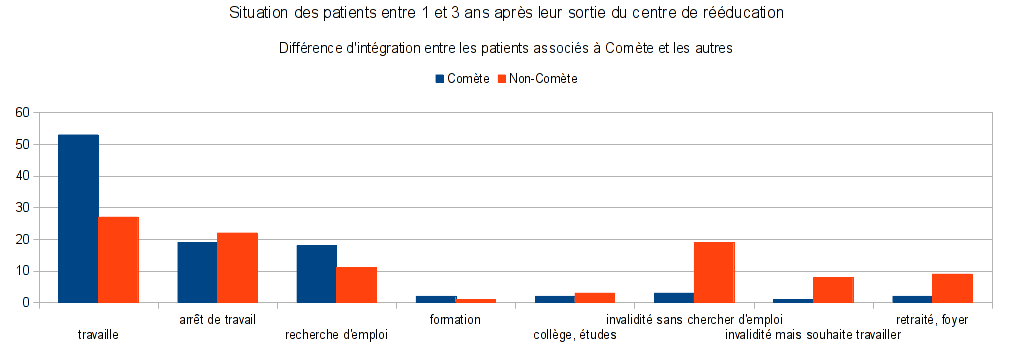
\includegraphics[scale=0.6]{figures/difference_integration.png}
\centering
\caption{Impact de l'accompagnement par l'association Comète dans la réinsertion professionnelle}
\end{figure}




\subsubsection{Agir très précocement après une maladie ou un accident}

Il est également nécessaire après une maladie ou un accident de débuter rapidement les démarches de réinsertion professionnelle. Car l'avenir de cette réinsertion dépend très étroitement de la qualité des contacts établis avec le médecin du travail et l'employeur dès les premières semaines de l'arr\^et maladie.\\

Dans le centre de rééducation fonctionnelle Propara à Montpellier où une équipe Comète est installée, les démarches d'ouverture d'un dossier sont faites à partir du moment où le nouveau patient est admis dans l'h\^opital. Une fois que l'état du patient est plus stable, des contacts sont établis pour faciliter le plus rapidement possible la réinsertion professionnelle. Il est cependant requis que ce soit la personne elle-même qui prolonge la démarche, une fois invitée par l'équipe à se présenter dans le service. L'accueil du patient est alors réalisé en quatre phases :
\begin{itemize}
\item L'accueil du patient et l'évaluation de la demande : capacités de la personne, information sur les prestations proposées et les solutions possibles, etc.
\item L'élaboration du projet et l'évaluation de sa faisabilité : l'évaluation des capacités professionnelles, le bilan des acquis scolaires et professionnels, la construction du projet professionnel, la mise en relation éventuelle avec les opérateurs d'insertion ou le passage de relais aux Cap Emploi pour les personnes à la recherche d'un emploi.
\item La mise en oeuvre du plan d'action : pour un retour à l'emploi dans l'entreprise ; pour une reprise de formation ou pour une reprise d'études.
\item Le suivi du devenir des personnes.\\
\end{itemize}
